%__________________________________________________________________________________________ %
%-------------------------------------------PFC---------------------------------------------%
%__________________________________________________________________________________________ %


%%%%%%%%%%%%%%%%%%%%%%%%%%%%%%  PREAMBULO  %%%%%%%%%%%%%%%%%%%%%%%%%%%%%%%%%%%%%
% ----------------------Especificaciones de dise�o---------------------------- %

\NeedsTeXFormat{LaTeX2e}
\documentclass[12pt]{book}

\usepackage{a4}
\usepackage[Lenny]{fncychap}    % Estilos para capitulos
\usepackage{fancyhdr}           % Estilos para cabeceras
%\usepackage[spanish]{babel}
%usepackage[latin1]{inputenc}

% Para no tener problemas con las tildes
\usepackage[utf8]{inputenc}
\usepackage[spanish]{babel}

\usepackage{epsfig}
\usepackage{subfig}
\usepackage{epstopdf}
\usepackage{caption}
\usepackage{keyval}
\usepackage{graphicx}
\usepackage{float}              % Para poner las imags en cualquier sitio
\usepackage{listings}
\usepackage{color}
\usepackage{textcomp}
\usepackage{verbatim}
\usepackage{exceltex}



\definecolor{listinggray}{gray}{0.98}
\definecolor{lbcolor}{rgb}{0.98,0.98,0.98}
\lstset{
	backgroundcolor=\color{lbcolor},
	tabsize=3,
	rulecolor=,
	language=matlab,
	basicstyle=\footnotesize\sffamily,
	aboveskip={1.5\baselineskip},
	belowskip={1.5\baselineskip},
	columns=fixed,
	showstringspaces=false,
	extendedchars=true,
	breaklines=true,
	prebreak = \raisebox{5ex}[5ex][5ex]{\ensuremath{\hookleftarrow}},
	frame=none,
	showtabs=false,
	showspaces=false,
	showstringspaces=false,
	identifierstyle=\ttfamily,
	keywordstyle=\color[rgb]{0,0,1},
	commentstyle=\color[rgb]{0.133,0.545,0.133},
	stringstyle=\color[rgb]{0.627,0.126,0.941},
}

\usepackage[numbers,sort&compress,comma]{natbib}	% Modo de poner la bibliograf�a
\usepackage{verbatim}      %  \begin{comment}...\end{comment}
\usepackage{subeqnarray}   % equationarray with numbers 1a, 1b, ...
\usepackage{bbm}           % Para s�mbolo tipo n�meros reales. Ej: \bbm{R}
\usepackage{longtable}     % Para tablas largas de m�s de una p�gina
\usepackage{rotating}
\usepackage{psfrag}        % Para cambiar fragmentos de text en .eps por otro en latex
\usepackage{pifont}        % Para otros s�mbolos
\usepackage{fancybox}      % Para encuadrar texto en recuadros
\usepackage{amsmath}       % Mejora la calidad de las formulas
\usepackage{amsfonts}
\usepackage [linktocpage]{hyperref}      % Para enlaces de hipertexto
\usepackage{amssymb,amsfonts}
\usepackage{multirow}
\usepackage{booktabs}
\usepackage{color}
\usepackage{longtable}
\usepackage{float}
\usepackage{array}




\setcounter{tocdepth}{2}             % toc = table of contents. Para definir niveles del �ndice
\setcounter{secnumdepth}{5}          % Hasta cu�ndo se enumeran los caps, seccs, etc


\setlength{\topmargin}{-1.1cm}        % margen por arriba
\setlength{\parskip}{\baselineskip}
\setlength{\parskip}{0.3cm}          % Espacio entre parrafos
\setlength{\textwidth}{16.5cm}       % Ancho del �rea imprimible	
\setlength{\evensidemargin}{-0.4cm}  % Margen izdo en p�ginas pares
\setlength{\oddsidemargin}{0.3cm}    % Margen izdo en p�ginas impares
% evensidemargin = -oddsidemargin !!!

\setlength{\headsep}{1.0cm}
\setlength{\headheight}{3ex}
\setlength{\footnotesep}{5mm}
%\setlength{\mathindent}{1.0cm}       % Controla el espacio entre margen y ec si no est� centrada


%%% Definitionen f�r Fancy Headings
%\renewcommand{\baselinestretch}{3mm}
%\renewcommand{\labelenumi}{\roman{enumi}.}
%\renewcommand{\chaptermark}[1]{\markboth{#1}{}}
%\renewcommand{\sectionmark}[1]{\markright{\thesection\ #1}{}}
\renewcommand{\labelitemi}{$\bullet$}
\renewcommand{\labelitemii}{$\diamond$}
\renewcommand{\labelitemiii}{$\cdot$}

\lhead[\fancyplain{}{\thepage}]{\fancyplain{}{\sl\nouppercase\rightmark}}
\rhead[\fancyplain{}{\sl\nouppercase\leftmark}]{\fancyplain{}{\thepage}}
\cfoot{}
\pagestyle{fancyplain}  		% normale Kopfzeile; ohne Seitenzahl: empty

% Formato de capitulos
\ChTitleVar{\sf\Huge} % Tama�o de la letra del nombre del cap
\ChTitleAsIs


%%% Comando para quitar encabezado y pie de las pag en blanco
\newcommand{\clearemptydoublepage}
{\newpage{\pagestyle{empty}\cleardoublepage}}

\newcommand{\R}{\mathbb{R}}
\newcommand{\x}{\mathbf{x}}
\newcommand{\grad}{\hspace{-2mm}$\phantom{a}^{\circ}$} %para los grados centigrados

%%% Abstract
\newenvironment{abstract}
{\begin{center}
		\begin{minipage}{0.8\textwidth}
			\slshape}
		{\end{minipage}
	\end{center}}
	
	
	\typeout{ }
	\typeout{----------------------------------------------------------------------}
	\typeout{ }
	
	



%%%%%%%%%%%%%%%%%%%%%%%%%%%%%%  DOCUMENTO  %%%%%%%%%%%%%%%%%%%%%%%%%%%%%%%%%%%%%
%-------------------------Cuerpo del documento---------------------------------%


\begin{document}
	\renewcommand{\contentsname}{Contents}
	\renewcommand{\listfigurename}{List of figures}
	\renewcommand{\listtablename}{List of tables}
	\pagenumbering{roman}    % Numeraci�n de p�ginas con num romanos
	\setcounter{page}{1}      % Establece la siguiente p�gina como la 1
	\begin{titlepage}
\label{ch:cover}
\begin{center}

{\Large\textsc{Telecomunication Engeneering}}


Department:  \\ Signal Theory, Telematics and Communications

\textbf{University of Granada}


\vspace{0.5cm}

\begin{figure}[h]
	\centering
	
\epsfig{file=imagenes/ugr, width=7cm}
	\label{fig:ugr}
\end{figure}


\vspace{0.5cm}
\textbf{Master thesis}


\vspace{0.9cm}


{\Huge\textbf{Comparison of Posturographic Body-sway Measurements with Inertial Data of Parkinson Patients }}


\end{center}


\vspace{1.5cm}
\textbf{Written by:}  \hfill \textbf{Supervised by:}

Ver\'onica Torres S\'anchez \hfill    D. Juan Manuel Górriz Sáez(UGR)

							\hfill	  D. Javier Ramírez Pérez de Inestrosa (UGR)
							
							\hfill    D. Alberto Olivares Vicente (UMU)
							
							\hfill	  D. Kai Bötzel (UMU)


\end{titlepage}
		% Inclu�mos la portada en espa�ol
	\clearemptydoublepage
	
	%Declaración
%--------

\begin{titlepage}
\label{ch:Statement}
\vspace{2cm}

\noindent  D. Alberto Olivares Vicente, profesor  del dpto. de Teoría de la Señal, Telemática y Comunicaciones, como director del Proyecto Fin de Carrera de Dª. Verónica Torres Sánchez,

\vspace{2cm}
\noindent Informan:

\vspace{1.5cm}
\noindent Que el presente trabajo, titulado:

\noindent \textbf{Comparison of Posturographic Body-sway Measurements with Inertial Data of Parkinson Patients.}

\noindent Ha sido realizado y redactado por el mencionado alumno bajo nuestra dirección, y con esta fecha autorizamos a su presentación.
\vspace{3.5cm}

\noindent Granada, a 20 de julio de 2015 Fdo:

\vspace{6.5cm}
\noindent D. Alberto Olivares Vicente    \hfill   D. Juan Manuel Górriz Sáez

\end{titlepage}       % Incluimos la declaración del proyecto
	\clearemptydoublepage
	\begin{titlepage}
\label{ch:acknowledgements}
{ \huge \bfseries Acknowledgements \\[0.4cm] }


First and foremost, I would like to thank Dr Alberto Olivares Vicente and Juan Manuel Górriz Sáez for supervising this work, his assistance and most especially for his continuous motivation and encouragement.

Thanks to Robin Weiss for his suggestions, his great ideas and knowledge, his jokes when the work was being  hard and, in short, for helping me along this Project.

Special thanks go to my friends for valuing my work, encouraging me every day, their advices and making me smile with their crazy things. Of course, many thanks go to my friend and flatmate, for putting up with me in the work nights and making to laugh with their positive music .

Finally, I am deeply grateful to my family, for giving me the opportunity to study, respecting all my decisions and their motivation and affection.


\end{titlepage}       % Incluimos agradecimientos
	\clearemptydoublepage
	\begin{titlepage}
\label{ch:abstract}
{ \huge \bfseries Abstract \\[0.4cm] }

\end{titlepage}       % Incluimos resumen
	\clearemptydoublepage
	
\begin{titlepage}
\label{ch:abbrevations}
{ \huge \bfseries Abbrevations \\[0.4cm] }

\textbf{APA}: Anticipatory postural adjustments

\textbf{SIPBA}: Signal processing and Biomedical Applications

\textbf{FP}: force plate

\textbf{GW}: Gait Watch

\textbf{QS}: Qualysis System

\textbf{PD}: Parkinson’s disease

\textbf{IMU}: Inertial Measurement Unit

\textbf{MIMU}: Magnetic Inertial Measurement Unit

\textbf{EMG}: Electromyography

\textbf{MEMS}: Microelectromechanical Systems

\textbf{LTSD}: Long Term Spectral Detector

\textbf{FSD}: Framed Spectrum Detector

\textbf{COP}: center of pressure

\textbf{AP}: Antero-posterior

\textbf{ML}: Medio Lateral

\textbf{FIR}: Finite Impulse Response.


\end{titlepage}       % Incluimos abreviaciones
	\clearemptydoublepage
	
	\tableofcontents          % Pone índice
   \listoffigures		   	% Crea la lista de figuras
   \listoftables			% Crea la lista de tablas
	\clearemptydoublepage

	

	\clearemptydoublepage
	\chapter{Introduction}
\label{ch:Introduction}

\section{General}

\subsection{Parkinson's Disease}

According to Patients Medical \cite{patients_medical_definition_2014}, \begin{quote}``Parkinson's disease is a progressive, neurodegenerative disease that occurs when the neurons within the brain responsible for producing the chemical dopamine become impaired or die. Dopamine is essential for the smooth control and coordination of the movement of voluntary muscle groups. Once approximately 80\% of the brain's dopamine producing cells no longer function, the symptoms of Parkinson's disease begin to appear. [\dots] Parkinson's disease may be termed as a progressive movement disorder that is distinguished by marked slow movements, tremors, and unstable posture.''\end{quote}

Especially in advanced stages of the Parkinson's disease (PD)\nomenclature{PD}{Parkinson's disease} many patients exhibit an episodic, brief inability to step that delays gait initiation or interrupts ongoing gait. This phenomenon is called freezing of gait and is often associated with an alternating shaking of the knees, called knee trembling. However, these clinical signs of balance or gait problems are not evident in early stages of the disease \cite{mancini_anticipatory_2009}\cite{jacobs_knee_2009}.

\subsection{Anticipatory Postural Adjustments}

A major challange to the human ballance control system is the fact that we are bipeds having only one foot in contact with the ground while walking, and that two-thirds  of our body mass is located two-thirds of body height above the ground \cite{halliday_initiation_1998}. Thus, to induce stable gait anticipatory postural adjustments (APAs)\nomenclature{APAs}{Anticipatory Postural Adjustments} are necessary. The Encyclopedia of Neuroscience \cite[p.133]{woollacott_anticipatory_2009} defines APAs as "A predictive motor response that acts to counter, in a preemptive manner, the postural destabilization associated with a forthcoming movement." As seen in Figure \ref{fig:APAoverview} the centre of body mass (COM)\nomenclature{COM}{Centre of Mass} is accelerated forward and laterally over the stance foot to make sure that the body does not fall laterally toward the stepping foot during the swing phase \cite{woollacott_anticipatory_2009}.  The curve of the centre of pressure (COP)\nomenclature{COP}{Centre of Pressure} is divided in three periods. Period S1 indicates the uncoupling of the COP and COM as the COP moves posteriorly and toward the intended stepping limb. Then, in the S2 period, the COP displaces mediolaterally toward the stance foot. Finally, during the S3 period the COP moves anteriorly under the stance foot \cite{hass_gait_2005-1}.

\begin{figure}
	\centering
	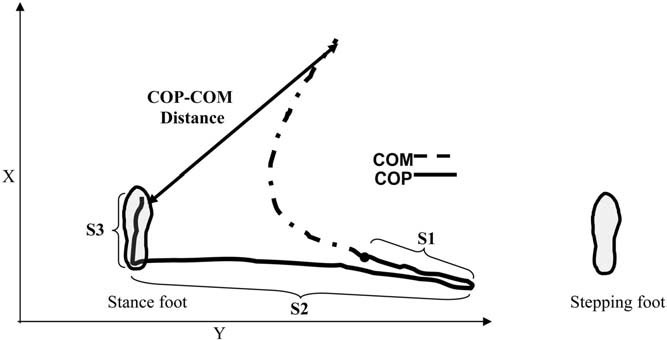
\epsfig{file=images/APA_overview, width=9cm}
	\caption{Anticipatory Postural Adjustments during forward-oriented gait initiation when stepping with the right foot \cite{hass_gait_2005-1}.}
	\label{fig:APAoverview}
\end{figure}


\section{Goals}

The goal of the project was to analyse anticipatory postural adjustments prior to step inition and subsequently build a classifier using MATLAB, which is fed with data from both a force plate and a magnetic inertial measurement unit (GaitWatch \cite{olivares_vicente_gaitwatch_2013}) to distinguish between Parkinson patients and healthy subjects. To gather the data the subject stood in front of the force plate. Then the GaitWatch and force plate record was started and the subject made a step onto the force plate. After standing a variable time of two to ten seconds the subject left the force plate, made a few steps, turned left und stopped in front of it again. This sequence was repeated ten times.


\section{Motivation}

Advanced PD can increasingly diminish quality of life, since patients are dependent on help from others to accomplish daily tasks. New drugs are currently being developed and are expected to decelerate or stop the course of the disease in early stages \cite{botzel_motivation_2014}. Thus, a quantitative PD classification enabling early diagnosis of the disease could optimise early treatment and could help to validate new treatment methods. Additionally, an objective evaluation of longterm treatment success was ensured.


\section{State of the art}

There are several methods and devices to assess Parkinson's disease and to analyse anticipatory postural adjustments. They differ in terms of practicability, accuracy, validity, portability, and cost. The state of the art at the beginning of the project is described below.

\subsection{Rating scales}

A commonly used rating scale is the Unified Parkinson’s Disease Rating Scale (UPDRS),\nomenclature{UPDRS}{Unified Parkinson’s Disease Rating Scale} which is a short test performed by a physician \cite{klerk_long-term_2009}. The patient is rated on 31 different items (see Table \ref{tab:UPDRS}) with a score of 0 (normal) to 4 (severely affected). Another method is the rough, but widely utilised and accepted Hoehn and Yahr scale (HY)\nomenclature{HY}{Hoehn and Yahr scale}. Parkinsonian motor impairment is categorised in 5 stages: Unilateral (Stage 1) to bilateral disease (Stage 2) without balance difficulties, to the presence of postural instability (Stage 3), loss of physical independence (Stage 4), up to being wheelchair- or bed-bound (Stage 5) \cite{goetz_movement_2004}. Without the need of complex technical devices these tests are relatively simple to perform. \citeauthor{klerk_long-term_2009} \cite{klerk_long-term_2009} mentioned their disadvantages, including subjectivity, short observation periods, and unfamiliarity of the environment that both rating methods bring along.

\begin{table}[h]
\begin{tabular}{lll}
\hline
Mentation, mood & Activities of daily & Motor examination \\
and behavior & living & \\
\hline
Intellectual impairment & Speech & Speech \\

Thought disorder & Salivation & Facial expression\\

Depression & Swallowing & Tremor at rest \\

Motivation/initiative & Handwriting & Action or postural tremor of hands \\

& Use of eating utensils & Rigidity \\

& Dressing & Finger taps\\

& Hygiene & Hand movements\\

& Turning in bed & Rapid alternating movements of hands\\

& Falling & Food agility\\

& Freezing when walking & Arising from chair \\

& Walking & Posture\\

& Tremor & Gait\\

& Sensory Complaints & Posture stability\\

& & Body bradikinesia and hypokinesia \\
\hline
\end{tabular}
\caption{Unified Parkinson's Disease Rating Scale items adapted from \cite{herndon_handbook_2006}.}
\label{tab:UPDRS}
\end{table}

\subsection{Instrumentation}

In addition to the aforementioned subjective rating scales, there are different devices used to quantify gait and posture and assess them objectively. All of them come with certain pros and cons. The following devices have been used:

\subsubsection{Electromyographs} Electromyography is a technique for evaluating the electrical activity of skeletal muscles. Successive action potentials generated by muscle cells are measured, by means of needle electrodes inserted into the muscles, and displayed on a cathode-ray oscilloscope. Thus medical abnormalities can be detected. The instrument used to capture the visual recording, termed electromyogram, is called electromyograph \cite{encyclopedia_britannica_electromyography_2014}. Electromyography is constrained to clinical application only, but gives indication about the contribution of specific, individual muscles to APAs.

\subsubsection{Force plates} Force plates quantify the ground reaction force (GRF)\nomenclature{GRF}{Ground Reaction Force}, which is the force exerted to the human body by the ground. The GRF is a three-dimensional vector with three orthogonal components. One component along the direction of gravity, one parallel to the ground in the sagittal plane, and one parallel to the ground in the frontal plane. Those are vertical planes that divide the body in left and right halves, and ventral and dorsal sections, respectively. A force plate usually gives an electrical voltage proportional to the force in each of the three directions. Force plates can be characterised according to the following criteria: Sensitivity in Volts per Newton, crosstalk (indication of vertical force if a horizontal force is applied and vice versa), repeatability (similar results under the same load), and time- and temperature drift \cite{griffiths_principles_2006}. Froce plates are limited to clinical application, too. They have the advantage that they don't have to be calibrated.

\subsubsection{Inertial measurement units} Devices that use a combination of inertial sensors like accelerometers and gyroscopes are referred to as inertial measurement units (IMUs)\nomenclature{IMU}{Inertial Measurement Unit}. If they also include magnetic field sensors (magnetometers), they are called magnetic inertial measurement units (MIMUs)\nomenclature{MIMU}{Magnetic Inertial Measurement Unit}. With these devices the orientation of the body can be obtained with up to nine degrees of freedom, provided that triaxial accelerometers and magnetometers are used, respectively \cite{olivares_vicente_signal_2013}.

\begin{itemize}

\item \textsc{Accelerometers} measure the acceleration of an object relative to an inertial frame. Since acceleration cannot be measured directly, the force exerted to a reference mass is obtained and the resultant acceleration is computed according to Newton's second law $ \mathbf{F} = m \cdot \mathbf a $ \cite{encyclopedia_britannica_accelerometer_2014}.

\item \textsc{Gyroscopes} measure angular velocity and are based on the Coriolis Effect. By means of integration of the angular velocity the rotation angle is obtained \cite{olivares_vicente_signal_2013}.

\item \textsc{Magnetometers} measure the strength and the direction of the magnetic field in a point in space, using the relationship between magnetic fields, movement and induced currents \cite{olivares_vicente_signal_2013}.
 
\end{itemize}
MIMUs are portable and relatively inexpensive. They can be easily attached to the body and thus allow non-clinical longterm application. Their drawbacks are complex calibration procedures and drift behaviour over time, depending on intensity and duration of the movement. Hence, in order to maintain a satisfactory degree of precision, periodical recomputation of the calibration parameters is required \cite{olivares_vicente_signal_2013}.

\subsection{Classification}

There are several research works in the literature dealing with APA analysis and PD classification, as the evaluation of posture and gait are key components of the clinical evaluation of PD \cite{palmerini_classification_2013}.

\citeauthor{klerk_long-term_2009} \cite{klerk_long-term_2009} developed a measurement system called PD Monitor, implementing an Activity Classifier that quantifies tremor and bradykinesia in the arm, thigh, and trunk, in an ambulant way and over long periods of time. They validated their measurements with video records, which were rated by physicians using the UPDRS and concluded that ``the PD monitor can be used for a detailed evaluation of the PD motor symptoms in order to optimize treatment.'' \cite{klerk_long-term_2009}.

\citeauthor{mancini_anticipatory_2009} \cite{mancini_anticipatory_2009} found that the 11 untreated early-to-middle stage Parkinson's patients that took part in their study have a significantly smaller peak COP displacement towards the stepping leg and peak trunk acceleration towards the stance leg compared to the 12 age-matched healthy control subjects. Even though step velocity and step length were not different. The results show that lateral APAs are impaired in early, untreated PD and that they are detectable with inertial sensors. As well as force plate-based, also acceleration-based extracted features can be used to detect impairments equally well. Due to the fact that the acceleration signal can be easily obtained via a sensor on a belt, no matter if in clinical or home environment, APA detection by means of accelerometers is considered as a useful way to characterise patients in early stage of PD without evident clinical symptoms. Additionally in \cite{mancini_anticipatory_2009} it is proposed to carry out further studies to determine the relationship between small APAs and the probability to develop start hesitation and freezing.

\citeauthor{palmerini_classification_2013} \cite{palmerini_classification_2013} states that PD classfication could deliver a tool to follow the progression of the disease during the entire course to examine the efficiency of treatment. They studied classification of PD subjects  using triaxial accelerometers on the lower back at L5 level and an ad hoc wrapper feature selection technique and achieved satisfactory accuracy of 93.75\%. Twenty early-mild PD subjects and 20 healthy age-matched control subjects had to perform two simple tests (quiet standing, Timed Up and Go test), in two evaluations over a 1-year follow-up, to test accuracy and robustness over time. As well as \cite{mancini_anticipatory_2009} they found that lateral dynamics i.e. range of motion are impaired in early-mild PD and suggested further investigation on validity of measures in later stages.

\section{Document structure}


	\clearemptydoublepage
	\chapter{Hardware Description}
\label{ch:Hardware}
Along this chapter we will introduce a general description of all devices used to data gathering for the development of this project.


It should be noted at this point that there are two clearly differentiated parts. In the first of them, we work with Force Plate and GaitWatch data, taking out their characteristic signals and synchronising them. In the second of them, we work jointly with Gait Watch and Qualisys System data for the purpose of comparing the accuracy in the calculated orientation angles.


\section{GaitWatch}

GaitWatch is an Inertial Measurement Unit (IMU) designed for gait monitoring of patients. It was developed by Prof. Dr. Med. Kai B¨otzel at the Department of Neurology of Ludwig-Maximilians University in Munich in conjunction with Dr. Alberto Olivares Vicente from the Department of Signal Theory, Telematics and Communications of the University of Granada. \cite{OlivaresBotzel2013}

The system is composed of the central processing unit and
a set of measuring units which are wired to it. The measuring units are 
placed in the patients’ thighs, shanks, arms and trunk.

The central processing unit has a microcontroller is in charge of gathering the data from the external measurement units and writing it to the memory card. So, this central unit is placed in the trunk inside a box and it contains an AL-XAVRB board with an AVRATxmega processor which contains the necessary embedded firmware to gather the data from all the measurement units and store it in a microSD card. Also, the trunk box contains some embedded magnetic and inertial sensors.

There are three different kinds of external units with the following components:
\begin{itemize}
	\item Type A (thighs and shanks): 
	\begin{itemize}
		\item IMU 5 from Sparkfun. IMU 5 contains an IDG500  biaxial gyroscope (from which only Y axis is actually used) with a measurement range of $\pm500deg/s$ and a $\pm3g$ triaxial accelerometer, ADXL335 .
	\end{itemize}
	\item Type B (arms):
	\begin{itemize}
		\item IDG500  biaxial $\pm500deg/s$ gyroscope.
	\end{itemize}
	\item Type C (trunk box):
	\begin{itemize}
		\item ADXL345  triaxial accelerometer with programmable range ($\pm16g/\pm8g/\pm4g/\pm2g$).
		\item IMU3000 triaxial gyroscope with programmable range ($\pm250/\pm500/\pm1000/\pm3000 (deg/s)$).
		\item Micromag3  triaxial magnetometer ($\pm11Gauss$).
	\end{itemize}
\end{itemize}


\section{Force Platform}

\section{Qualisys System}
	\clearemptydoublepage
	\chapter{Synchronisation}
\label{ch:Synchronisation}

\section{Introduction and chapter's structure}
One of the most important aspects whether you have data acquired from multiples devices or channels is the synchronisation. If these data are not appropriately correlated or synchronised, the analysis and conclusions from your use will be erroneous. Also, it’s very important doing all automatically when you have a data on a broad scale.
Therefore, the following sections explain how the information has been obtained and processed automatically, as well as what features have been calculated to characterise the movements of the patients and to carry out the synchronisation between the Force Plate signals and GaitWatch signals. This content is superficially depicted in figure XX.

\begin{figure}[H]
	\centering
	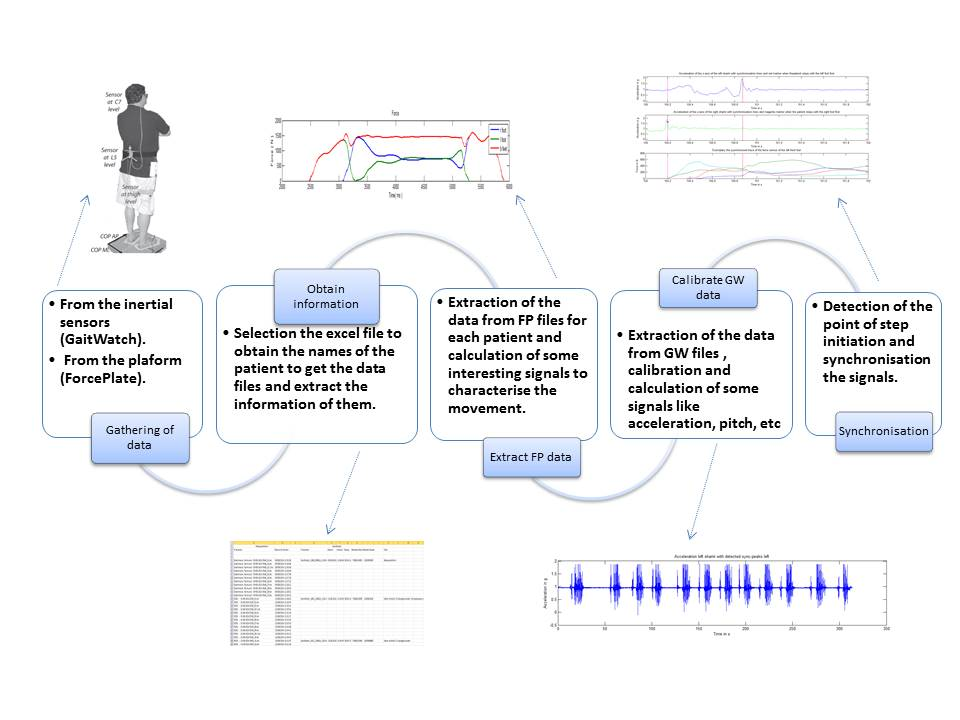
\epsfig{file=imagenes/diagramSynchronisation, width=7cm}
	\caption{Diagram of the Synchronisation's progress.}
	\label{fig:arte1}
\end{figure}

\section{Data gathering Protocol}
Prior to start of data gathering, it’s necessary to set up the protocol for procedure that patients have to carry out while the data are recorded. The establishing this procedure is very important so that the synchronisation works properly because we have to identify a clear movement in both signals to match one signal with the other at the same time.
In addition, the realised movements must be representatives to obtain conclusive data which help us to extract characteristics for the purpose of identify differences between patients and control subjects subsequently.

The steps followed by the patients are detailed hereafter:

1.	Subject stands in front of the Force Plate.

2.	Gait watch record starts for data gathering.

3.	Force plate record starts for data gathering.

4.	Subject makes a step onto the platform.

5.	Subject stands on the platform a variable time between 2 and 10 seconds.

6.	Subject makes some step  forward and turns left to stand in front of the platform again.

This procedure is repeated ten times by each subject in order to characterise better the movement made.
It’s important to clarify that the GaitWatch recording contains all these ten episodes ( in other cases more) and the platform recording only contains one episode each. So, this is a fact that we have to consider to do the synchronisation.


\section{Design of developed code  in Matlab}
	\subsection{Selection, reading and obtaining of information from the excel file}
	\subsection{Extraction of the forceplate data}
	\subsection{Calibration of the GaitWatch data}
	\subsection{Synchronisation}	
\section{Results discurssion}		

	
	\clearemptydoublepage
	\bibliographystyle{unsrt}
	\bibliography{biblio}
	
	\clearemptydoublepage
\end{document}